%%% FILE WITH ALL TABLES DEFINITIONS %%%

%%% EXAMPLE TABLE %%%
\renewcommand{\Tabladeejemplo}{
    \begin{table}[h]
        \centering
        \caption{Caption for the table.}
        \label{tab:example_table}
        \begin{tabularx}{\textwidth}{XXX} % Removed the extra brackets
            \toprule
            Column 1 & Column 2 & Column 3 \\ \midrule
            Data 1 & Data 2 & Data 3 \\
            Data 4 & Data 5 & Data 6 \\
            \bottomrule
        \end{tabularx}
    \end{table}
}

%%% APPROVAL TABLE %%%
\renewcommand{\approvaltable}{
    \begin{center}
        \begin{table}[ht]
            \begin{tabularx}{\textwidth}{lXXX}
            \toprule
            \textbf{Title}        & \multicolumn{3}{l}{\textbf{FYS DRD and Guidelines}}   \\ \midrule
            Issue Number & 1                      & Revision Number  & 0 \\ 
            Author       &  Edgar Hernandez Recio                      & Date             &   \\ 
            Approved By  &                        & Date of Approval &   \\ 
            \bottomrule
            \end{tabularx}
            \label{tab:approval}
        \end{table}
    \end{center}
}

%%% APPROVAL TABLE %%%
\renewcommand{\changelogtable}{
    \begin{center}
        \begin{table}[ht]
            \begin{tabularx}{\textwidth}{lXXX}
            \toprule
            Reason for change   & Issue Nr  & Revision Number   & Date  \\ \midrule
            First release       & 1         & 0                 &       \\ 
            Second release      & 2         & 0                 &       \\
            \bottomrule
            \end{tabularx}
            \label{tab:change_log}
        \end{table}
    \end{center}
}

%%% APPROVAL TABLE %%%
\renewcommand{\recordtable}{ 
    \begin{center}
        \begin{table}[ht]
            \begin{tabularx}{\textwidth}{lXXX}
            \toprule
            \textbf{Issue Number}   & \multicolumn{3}{l}{\textbf{Revision Number}}  \\ \midrule
            Issue Number            & 1         & Revision Number   & 0             \\ \midrule
            Reason for change       & Date      & Pages             & Paragraph(s)  \\ \midrule
            First release           &           &                   &               \\
            Second release          &           &                   &               \\
            \bottomrule
            \end{tabularx}
            \label{tab:change_record}
        \end{table}
    \end{center}
}

%%% DISTRIBUTION TABLE %%%
\renewcommand{\distributiontable}{
    \begin{center}
        \begin{table}[ht]
            \begin{tabularx}{\textwidth}{X}
            \toprule
            \textbf{Disclaimer} \\ \midrule
            This document has been prepared for use by the Fly Your Satellite! PoCat Lektron team.\\
            \textbf{This document shall be considered confidential and not to be distributed further without permission of ESA Education, and the authors.}   \\ \bottomrule
            \end{tabularx}
            \label{tab:distribution}
        \end{table}
    \end{center}
}

%%% Table for the sensors and actuators %%%
\renewcommand{\sensorsactuators}{
    \begin{table}[h]
        \centering
        \begin{tabular}{ll}
            \hline
            \textbf{Sensors}      & \textbf{Actuator}     \\ \hline
            Gyroscope    & Magnetorquer \\
            Photodiodes  &              \\
            Magnetometer &              \\ \hline
        \end{tabular}
    \end{table}
}
%%% Table for the magnetorquer description %%%
\renewcommand{\magnetorquercharacteristics}{
    \begin{table}[htbp]
    \centering
        \begin{tabularx}{0.9\linewidth}{X c c c c}
            \toprule
            \textbf{Board} & \textbf{Turns} & \textbf{Max moment (A$\cdot$m$^2$)} & \textbf{Dimensions (mm$\times$mm)} & \textbf{Layers} \\
            \midrule
            Top & 42$\times$layer & $9.17 \times 10^{-4}$ & 32 $\times$ 32 & 4 \\
            Bottom \& Lateral & 38$\times$layer & 0.0017 & 32 $\times$ 32 & 4 \\
            \bottomrule
        \end{tabularx}
    \end{table}
}
\section{Simulation model}
To assist the AOCS design, verification and validation, a simulation model using mathlab code has been used. The
simulation is based on the Princeton Toolbox \cite{PrincetonToolbox}, which contains a set of functions and 
simulations initially created for CubeSats, that has been adapted to the PocketQube.

\subsection{PocketQube Model}
The mission is formed by two PQs, one using an L-band Radiometer and the other using a K-band radiometer. To model the PQ, a 3 dimensional cube has
been used, shown in \textit{Figure \ref{fig:PQmodel}}. This cube has the same dimensions as a PQ 5x5x5 cm$^2$ and the same mass as the PQs. Additionally, to apply the inertia of the PQs, the 
inertia matrix is taken into account in the simulation.\vspace{0.2em}

\noindent The satellites will be simulated in two different configurations, on the one hand in stowed configuration (without the anntennas deployed) and on the other
hand in deployed configuration. In the case of the L-band PQ the stowed configuration contains both the L-band antenna and communications antenna
stowed.
    \begin{figure}[H]
        \centering
        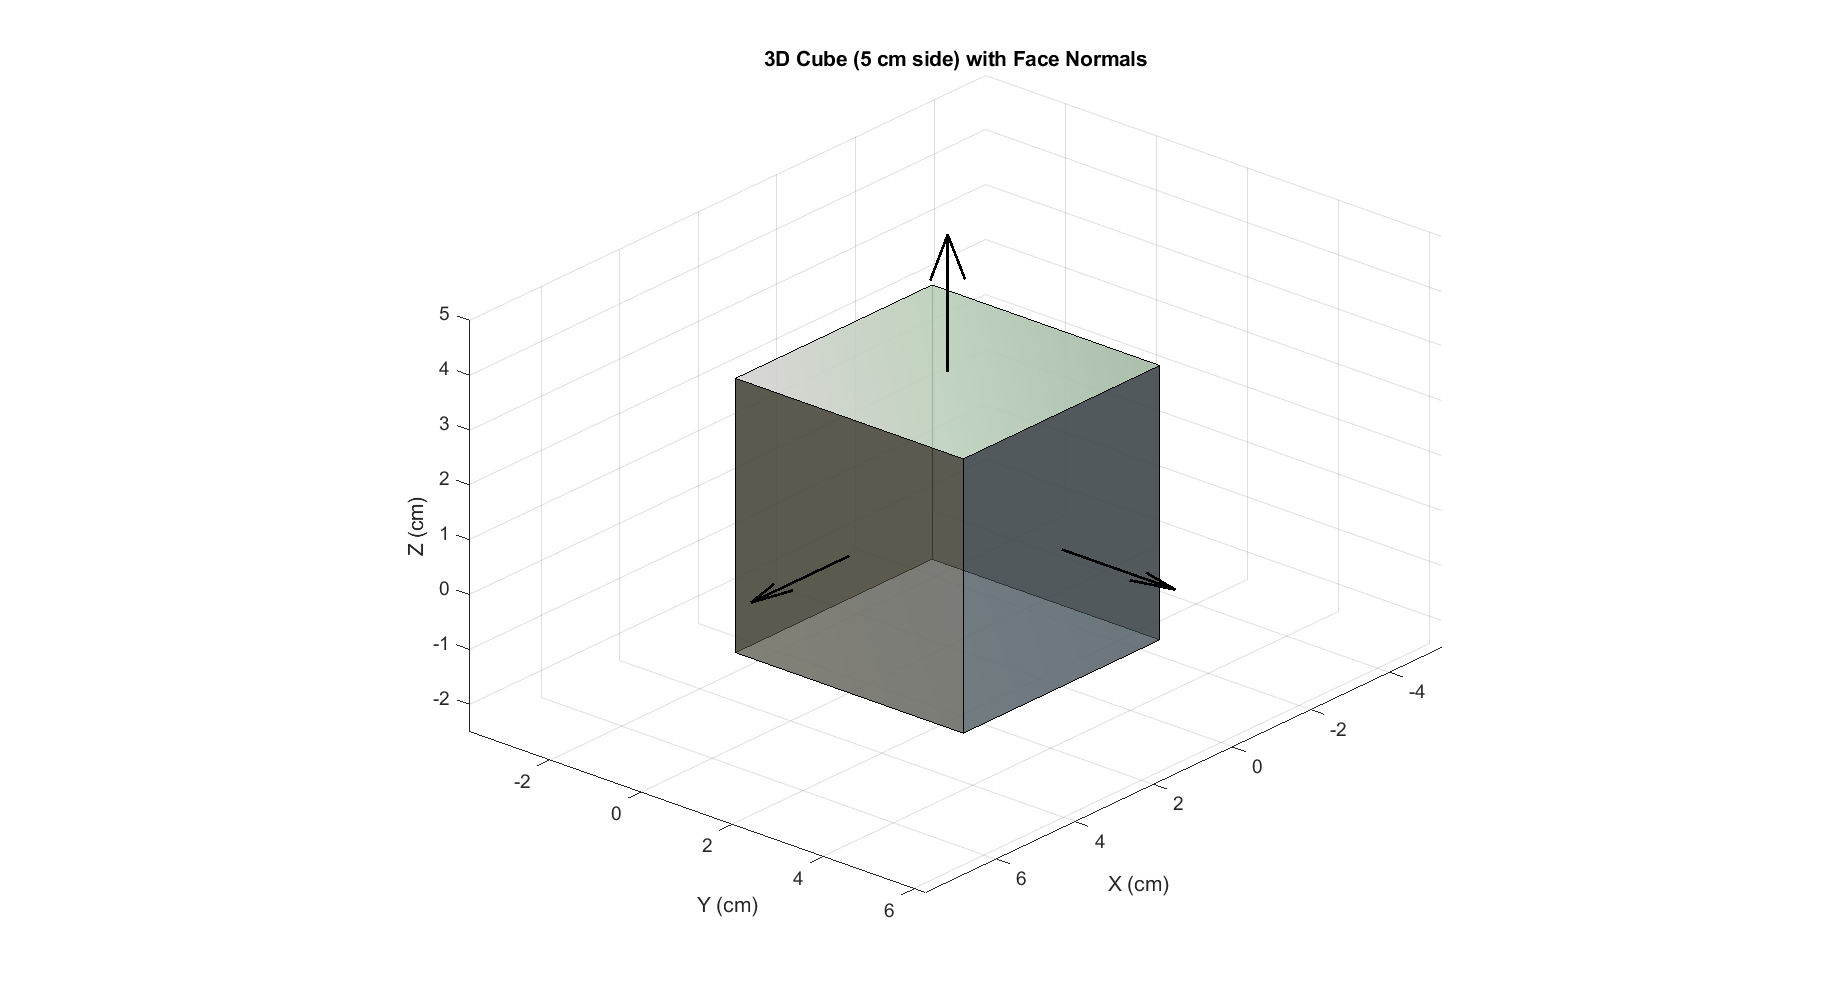
\includegraphics[width=0.8\linewidth]{res/img/3_simulation_performance/PQ model.png}
        \caption{PocketQube 3D model}
        \label{fig:PQmodel}
    \end{figure}

\subsection{Environmental model and asumptions}

\subsubsection{Reference framse}
\begin{itemize}
    \item \textbf{Earth Centered Inertial (ECI) frame:}\\
    The ECI frame is a global cartesian reference frame that has its origin at the centre of the
    Earth.
    \begin{itemize}
        \item X axis points to the Vernal Equinox.
        \item Y axis completes the set with the right-hand rule.
        \item Z axis aligned with the Earth's rotation axis.
    \end{itemize}

    \begin{figure}[H]
        \centering
        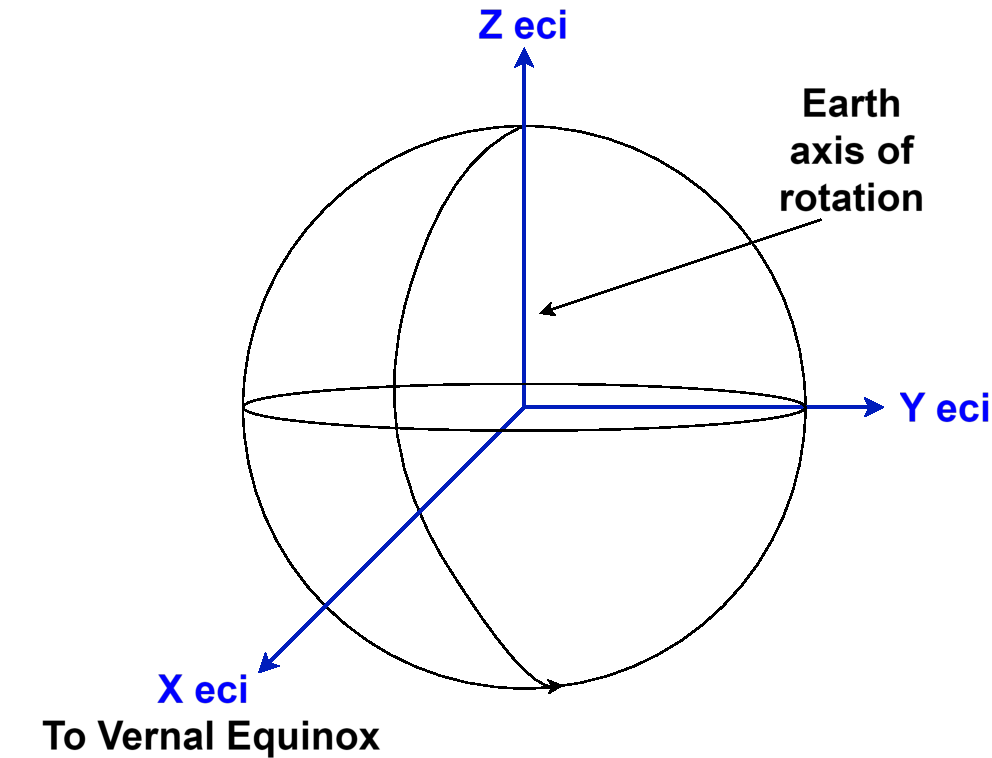
\includegraphics[width=0.4\linewidth]{res/img/3_simulation_performance/ECI frame.drawio.pdf}
        \caption{ECI frame representation}
        \label{fig:ECIframe}
    \end{figure}

    \item \textbf{Body frame:}\\
    The Body frame is a global cartesian reference frame that has its origin at the centre of
    the PQ.
    \begin{itemize}
        \item X axis aligned with the PocketQube width, parallel to the sliding plate and perpendicular
        to the direction of insertion into the PocketQube deployer.
        \item Y axis aligned with the PocketQube length, the direction of insertion into the
        PocketQube deployer and completing the right handed reference frame.
        \item Z axis aligned with the PocketQube height direction, pointing upwards from the
        sliding plate.

    \end{itemize}

    \begin{figure}[H]
        \centering
        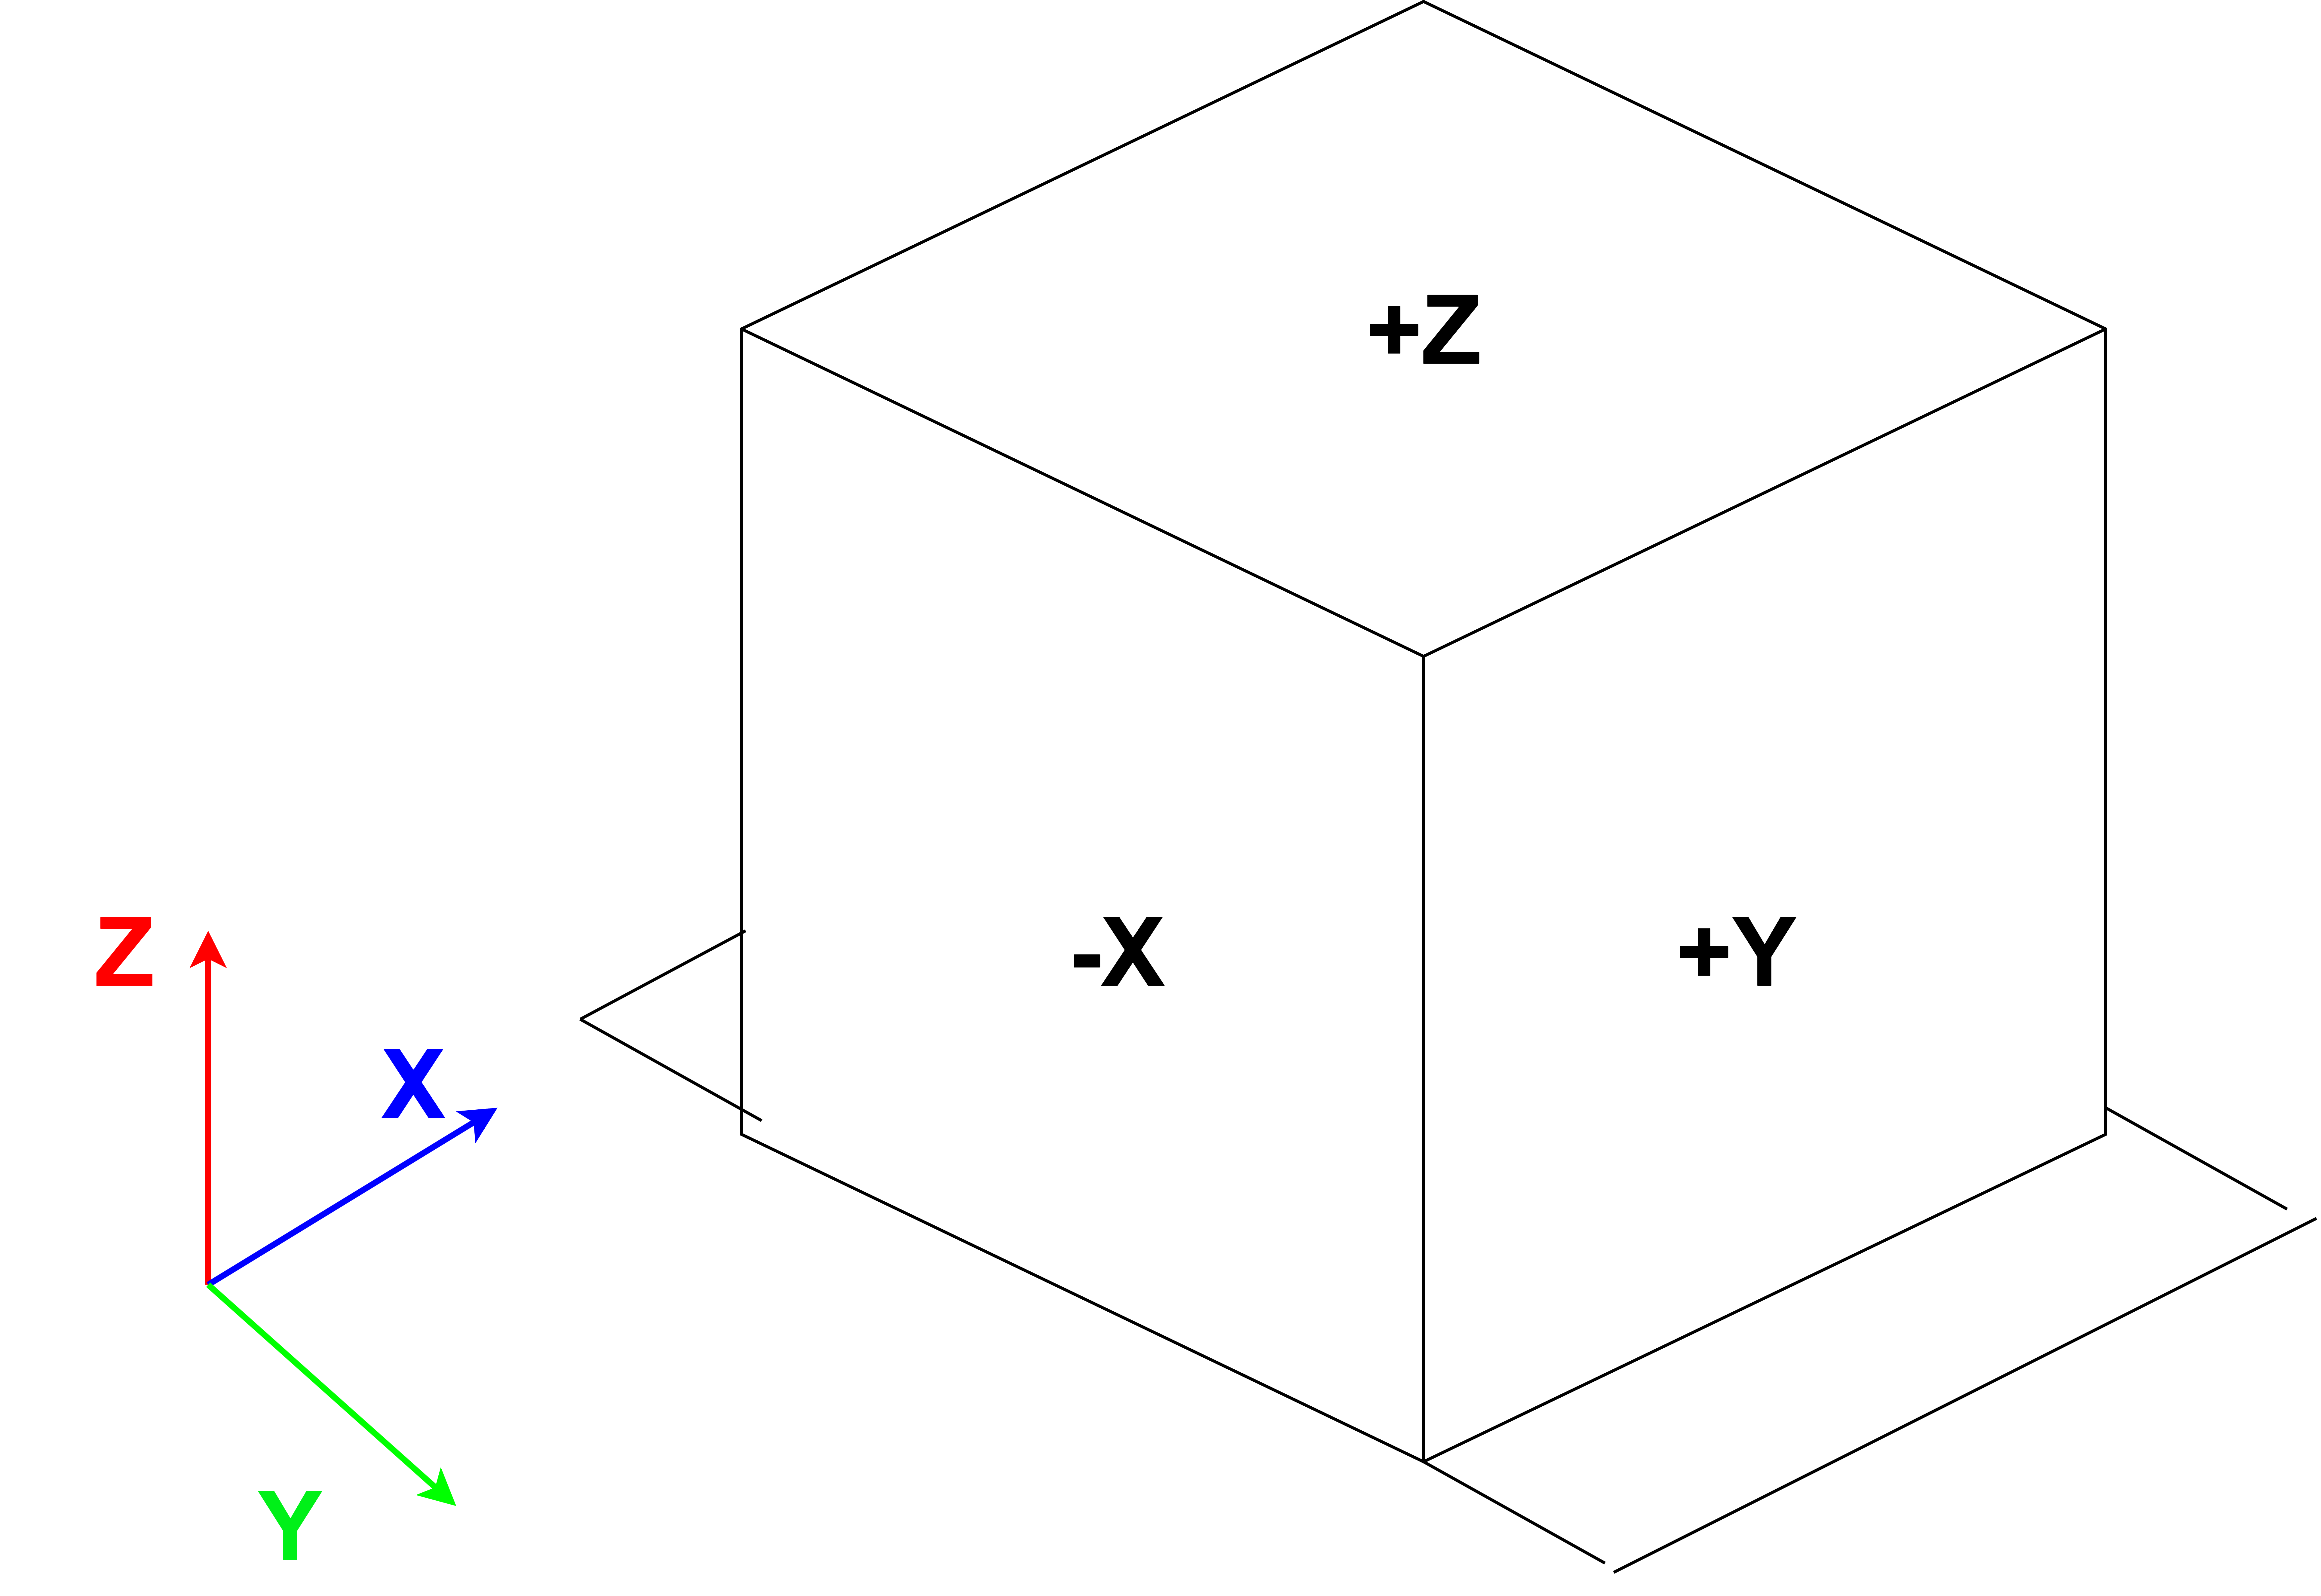
\includegraphics[width=0.4\linewidth]{res/img/3_simulation_performance/bodyframe.drawio.png}
        \caption{Body frame representation}
        \label{fig:ECIframe}
    \end{figure}

    \item \textbf{Local Vertical Local Horizontal (LVLH) Frame:}\\
    The LVLH Frame will be mainly used for results presentation in the Nadir pointing simulations. The frame is described as:
    \begin{itemize}
        \item X-Axis: Perpendicular to Y and Z, forming a right-handed coordinate system - Local Horizontal
        \item Y-Axis: Negative to the orbit normal, or in the direction of -h
        \item Z-Axis: Oriented in the direction of -r (points to center of Earth) - Local Vertical
    \end{itemize}

    \begin{figure}[H]
        \centering
        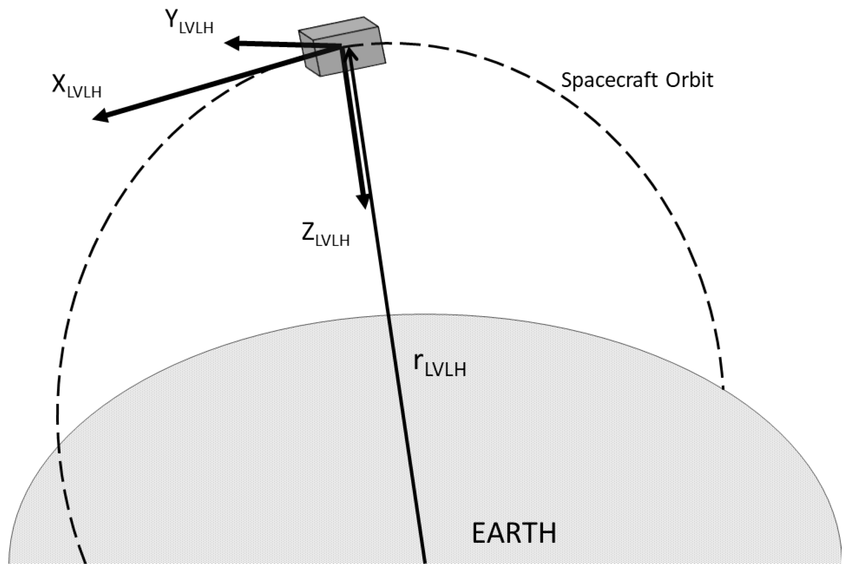
\includegraphics[width=0.4\linewidth]{res/img/3_simulation_performance/LVLH-Local-Vertical-Local-Horizontal-frame-definition.png}
        \caption{LVLH frame representation}
        \label{fig:ECIframe}
    \end{figure}
\end{itemize}

\subsubsection{Environmental models}
The following environmental models are used in the simulation:
\begin{itemize}
    \item \textbf{Earth's magnetic field model \cite{Tilted_Dipole}:} The Earth's magnetic field model used in the simulation is based
    on the Tilted dipole mode, which includes the effect of the dipole motion of the Earth.
    \item \textbf{Aerodynamic Drag model:} The simulation uses an aerodinamic drag model based on the Jacchia's 1970 model
    \cite{J70_atmosphere}. 
    \item \textbf{Radiation Pressure model:} The simulation includes the solar radiation pressure, the earth radiation
    pressure and the earth albedo pressure.
    \item \textbf{Gravity field model:} The simulation accounts for a point-mass gravity model.
\end{itemize}

\subsubsection{External disturbances}
The following external disturbances are considered in the simulation:
\begin{itemize}
    \item \textbf{Drag force:} 
    \item \textbf{Aerodynamic torques:} 
    \item \textbf{Gravity gradient torques:} 
    \item \textbf{Radiation Torques:} 
\end{itemize}

\subsection{Orbit and attitude kinematic propagators}

As for the Orbit propagator in the simulation, firstly, the used equations or motion are the Cowell'
form of the two body problem, using  disturbances. In addition, the integrator type used is the Runge-Kutta 4th order method.
As for the propagation of the parameters, they are done in the Earth Centered Inertial (ECI) frame.\vspace{0.2em}

\noindent The parameters included in the initial vector for describing the state of the satellite at the begining of the simulation are:

\begin{itemize}
    \item Satellite's position.
    \item Satellite's velocity.
    \item Satellite's attitude quaternion.
    \item Satellite's angular velocity.
\end{itemize}

\noindent Regarding the attitude representation of the satellite in the simulation, the mathematical expresion that will be used is the quaternion. During the
simulation the quaternion that will be used is the one representing the rotation fromt he body frame to the ECI frame. However, at the time to 
present the results the quaternion that will be used will be the one representing a rotation from the Local Vertical Local Horizontal (LVLH) frame to the ECI frame.

\subsection{Sensor and actuator models}
In this section all the models used for the sensors and for the actuators are described. It is assumed that all the sensors has been calibrated
and temperature characterized. A brief list of the sensors and actuators included in the PQ is presented below:

\sensorsactuators

\subsubsection{Gyroscope}
The model used to represent the gyroscope output given by \cite{Landis} is:

\begin{equation}
    \boldsymbol{\omega} = \boldsymbol{\omega_o} +\boldsymbol{b(t)}+\boldsymbol{n},
\end{equation}
where:
\begin{itemize}
    \item $\boldsymbol{\omega}$ is the measured angular velocity vector.
    \item $\boldsymbol{\omega_o}$ is the true angular velocity of the satellite.
    \item $\boldsymbol{b}$ is the bias term, modeled as a random walk process.
    \item $\boldsymbol{n}$ is a zero-mean Gaussian noise vector.
\end{itemize}
\subsubsection{Photodiodes}

The output of the photodiodes can be modeled as:

\begin{equation}
    \boldsymbol{v} = \boldsymbol{v_o(T)} + \boldsymbol{n}
\end{equation}

where:
\begin{itemize}
    \item $\boldsymbol{v}$ is the measured voltage output vector,
    \item $\boldsymbol{v_o(T)}$ is the true signal component that is dependent to the temperature $\boldsymbol{T}$ previously calibrated.
    \item $\boldsymbol{n}$ represents additive noise, typically modeled as zero-mean Gaussian noise.
\end{itemize}

\subsubsection{Magnetometer}

The magnetometer model is expressed as:

\begin{equation}
\boldsymbol{B}_{\text{meas}} = \left( \mathbf{C}_e \cdot \boldsymbol{B}_{\text{true}} \right) + \boldsymbol{b}_e + \boldsymbol{n}
\end{equation}

where:

\begin{itemize}
    \item $\boldsymbol{B}_{\text{meas}}$ is the measured magnetic field vector in the body frame.
    \item $\boldsymbol{B}_{\text{true}}$ is the true magnetic field vector in the body frame.
    \item $\mathbf{C}_e$ is the calibration matrix with errors.
    \item $\boldsymbol{b}_e$ is the sensor bias error vector.
    \item $\boldsymbol{n}$ is zero-mean Gaussian white noise with known variance.
\end{itemize}

\subsubsection{Magnetorquer}
The magnetorquers are simulated as a mathematical formula. The magnetorquers generate a magnetic moment depending on the injected intensity, therefore,
in the simulation this magnetic moment is calculated and later used to propagate the following attitude of the satellite with the other external disturbances.
The formula used for calculating the magnetic moment generated by the magnetorquers is:

\begin{equation}
    \boldsymbol{m}=I_o·N_{layers}·\sum_{i=1}^{N_{turns}}(l-2(i-1)(w+d))^2
\end{equation}

\noindent Where the $l$ is the length of the magnetorquer, the $w$ the width of the copper trail, the $d$ the distance between trails, $N_{layers}$ is the number
layers in which the magnetorquer is divided and $N_{turns}$ is the number of turns in the magnetorquer. The $I_o$ is the injected current, which is the input of the magnetorquer. 
The table below shows the characteristics of the magnetorquers used in the simulation:

\magnetorquercharacteristics



\subsection{Simulaton / model sampling times and frequencies}
The simulation time used is 2 seconds which corresponds to 0.5 Hz. This is due to the fact that the on board computer (OBC) used in the PQ
only has one thread to manage all the tasks, therefore, the sampling frequency has been chosen thinking in the worst case scenario. The 
sampling time of the sensors is the same one as the simulation time.

\section{Simulation performance campaign plan and results}

In this section the simulation results of the two different operational modes of the ADCS in the PQ are presented.

\subsection{Nadir Pointing Mode}

The objective of the Nadir Pointing is to point the Payload located at the top board of the PocketQube towards the Earth, so that 
the Payload can take measurements of the Earth. For this mode the following requirements have been defined:

\noindent \textit{The Absolute Performance Error (APE) of the Payload boresight shall be less than 20º with respect to the Y and X 
axes, which are the axes perpendicular to the boresight, and this requirement should be met for 95\% of the time.}

The PocketQube will be in deployed coniguration during the simulation.


\subsubsection{Assumptions and limitations}
The list below presents the different assumptions and aspects considered to perform the simulations.
\begin{itemize}
    \item \textbf{Orbit parameters}
    \begin{itemize}
        \item Inclination: 90 degrees
        \item Altitude: 500 Km
        \item Eccentricity: 0 degrees
        \item Initial satellite position: [ 6887 , 0 , 0 ] Km
        \item Initial satellite velocity: [ 0 , 0 , 7.6 ] Km/s
        \begin{figure}[H]
            \centering
            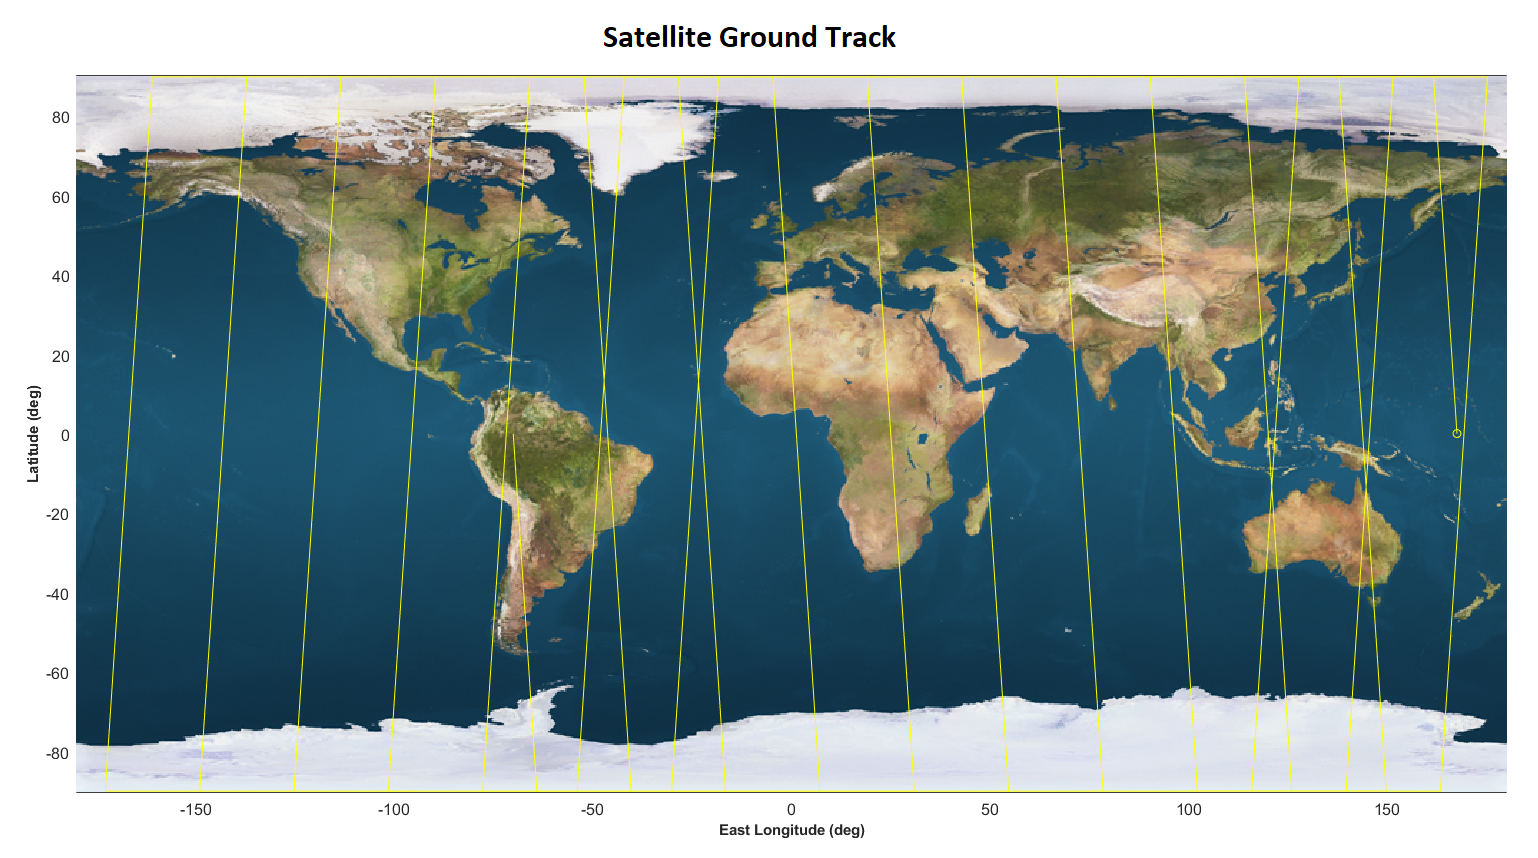
\includegraphics[width=0.8\linewidth]{res/img/3_simulation_performance/Sat_groundtrack.png}
            \caption{Ground track of the simulated PocketQube orbit}
            \label{fig:GTrack}
        \end{figure}
    \end{itemize}

    \item \textbf{Number of simuated orbits:} 10 orbits
    \item \textbf{Simulation starting date:} 05/04/2027 00:00:00 UTC
    \item \textbf{Simulation time step:} 2 seconds
\end{itemize}


\subsection{Detumbling mode}